%%% pilot.Rnw 

%% Author: emanuelheitlinger@gmail.com

\documentclass[12pt,a4paper]{article}
\usepackage[debugshow,final]{graphics}
\usepackage{hyperref}
\usepackage{float}
\usepackage{lscape} 
%\revision$Header: /home/ele/pilot_sanger/pilot.Rnw,v 1.1 2009/10/26 15:38:20 ele Exp $

\usepackage{/usr/share/R/texmf/tex/latex/Sweave}
\begin{document}

\setkeys{Gin}{width=1.25\textwidth}



%%%%##########################################################################



\title{The transcriptome of \textit{Anguillicoloides crassus}. Part A:
  Pilot-sequencing} \author{Emanuel G Heitlinger} \date{}
\maketitle

\section*{Abstract}
In preparation of high-throughput transcriptome sequencing of the
swimbladder nematode \textit{A. crassus} expressed sequence tags
(ESTs) were generated using traditional Sanger-technology. In total
945 reads from adult \textit{A. crassus} (5
libraries from 4 cDNA preparations) and 288
reads from liver-tissue of the host species \textit{Anguilla japonica}
(3 libraries from 3 cDNA preparations) were sequenced. After
base-calling an quality screening 452 of the
nematode and 195 of the host reads were of
sufficient quality for further processing.

115 of the nematode and
36 of the host reads were of sufficient
quality for submission to dbEST.

Additionally 13 sequences originating
from host-contamination had to be removed from the \textit{A. crassus}
data-set for submission to NCBI-dbEST, reducing it to
115 ESTs. Nevertheless the stringent quality
trimming and processing of raw reads, as summarized in the present
document, make the remaining ESTs a valuable resource for comparison
with future 454-sequencing-data.

\section*{Introduction}

After sampling adult and larval \textit{A. crassus} from the wild in
Taiwan and Germany the generation of cDNA libraries from small amounts
of starting material was made difficult to achieve for two reasons:
\begin{itemize}
\item The larvae are of small size and only available in limited
  numbers from the wild.
\item Adult worms consist predominantly of ingested host blood.
\end{itemize}

Therefore an amplification protocol for cDNA had to be used. As low
amounts of starting material and the use of these protocols could
produce unwanted contamination by amplification artifacts obtained
cDNA libraries were analyzed using traditional Sanger-sequencing.

\section*{Material and methods}

During sampling in Taiwan (sampling locations published in
\cite{heitlinger_massive_2009}) and Germany, single adult
\textit{A. crassus} were preserved in RNAlater(Quiagen, Hilden,
Germany), after their sex had been determined. Total RNA was extracted
from single, whole worms using the RNeasy kit (Quiagen, Hilden,
Germany), following the manufacturers protocol. Alternatively parts of
the liver of the host species \textit{Anguilla japonica}, which also
had been preserved in RNAlater were used for RNA extraction, following
the same protocol.

The Evrogen MINT cDNA synthesis kit (Evrogen, Moscow, Russia) was
then used to amplify mRNA transcripts according to the manufacturers
protocol. It uses an adapter sequence at 3' the end of a a poly
dT-primer for first strand synthesis and adds a second adapter
complementary to the bases at the 5' end of the transcripts by
terminal transferase activity and template switching. Using these
adapters it is possible to specifically amplify mRNA enriched for
full-length transcripts. The obtained cDNA preparations were
undirectionally cloned into TOPO2PCR-vectors (Invitrogen, Carlsbad,
USA) and TOP10 chemically competent cells (Invitrogen, Carlsbad, USA)
were transformed with this construct. The cells were plated on
LB-medium-agarose containing Kanamycin (5mg/ml), xGal
(5-bromo-4-chloro-3-indolyl-$\beta$-D-galactopyranoside) and IPTG
(Isopropyl-$\beta$-D-1-thiogalactopyranosid). After 24h of incubation
at $36\,^{\circ}\mathrm{C} $ cells were picked into 96-well
micro-liter-plates containing liquid LB-medium and Kanamycin (5mg/ml)
and incubated for another 24h. Subsequently 2ml of the cells were used
as template for amplification of the insert by PCR using the primers
\begin{description}
\item[Forward] M13F(GTAAAACGACGGCCAGT) and
\item[Reverse] M13R(GGCAGGAAACAGCTATGACC)
\end{description}
in a concentration of 10$\mu$M. The protocol for PCR cycling is shown
in table \ref{tab:PCR}.

\begin{table}[ht]
  \centering
  \begin{tabular}{lllll} 
    \textbf{Inital denaturation} &  $ 94\, ^{\circ}\mathrm{C} $ & 5min &  &\\ 
    \hline
    \textbf{Denaturation} &  $ 94\, ^{\circ}\mathrm{C} $ &30s& & \\ 
    \textbf{Annealing} &   $ 54\, ^{\circ}\mathrm{C} $ & 45s & 35 cycles &\\ 
    \textbf{Elongation} &   $ 72\, ^{\circ}\mathrm{C} $ & 2min &  &\\ 
    \hline
    \textbf{Filnal Elongation} &   $ 72\, ^{\circ}\mathrm{C} $ & 10min &\\ 
  \end{tabular}   
  \caption{PCR protocol for insert amplification}
  \label{tab:PCR}
\end{table}

Amplification products were controlled on gel and cleaned using SAP
(Shrimp Alkaline Phosphatase) and ExoI (Exonuclease I). Sequencing
reactions were performed using the BigDye-Terminator kit and
PCR-primers (forward or reverse) in a concentration of 3.5$\mu$M and
sequenced on an ABI 3730 DNA Analyzer (Applied Biosystems, Foster
City, California, USA).  For \textit{A. crassus} the following
libraries were prepared:
 
\begin{list}{\labeldescription}{\leftmargin = 5em}
  \setlength{\itemsep}{1pt} \setlength{\parskip}{1pt}
  \setlength{\parsep}{0pt}
\item[Ac\_197F:] Female from Taiwanese aquaculture
\item[Ac\_106F:] Female from Taiwanese aquaculture
\item[Ac\_M175:] Male from Taiwanese aquaculture
\item[Ac\_FM:] Female from Taiwanese aquaculture
\item[Ac\_EH1:] Same cDNA preparation as Ac\_FM, but sequenced by
  students in a practical
\end{list}

For \textit{Anguilla japonica} the following three libraries:
\begin{list}{\labeldescription}{\leftmargin = 5em}
  \setlength{\itemsep}{1pt} \setlength{\parskip}{1pt}
  \setlength{\parsep}{0pt}
\item[Aj\_Li1:] liver of an eel from aquaculture
\item[Aj\_Li2:] liver of an eel from aquaculture
\item[Aj\_Li3:] liver of an eel from aquaculture
\end{list}

The original sequencing-chromatographs ("trace-files") were renamed
according to the NERC environmental genomics scheme. "Ac" was used as
project-identifier for \textit{Anguillicoloides crassus}, "Aj" for
\textit{Anguilla japonica}. In \textit{Anguillicoloides} sequences
information on the sequencing primer (forward or reverse PCR primer
\textit{Anguilla japonica} sequences were all sequenced using the
forward PCR primer) was temporarily stored in the middle
"library"-field, resulting in names of the following form:\\
\texttt{Ac\_[\textbackslash{}d|\textbackslash{}w]\{2,4\}(f|r)\_\textbackslash{}d\textbackslash{}d\textbackslash{}w\textbackslash{}d\textbackslash{}d}\\
\texttt{Aj\_[\textbackslash{}d|\textbackslash{}w]\{2,4\}\_\textbackslash{}d\textbackslash{}d\textbackslash{}w\textbackslash{}d\textbackslash{}d}\\
The last field indicates the plate number (two digits), the row (one
letter) and the column (two digits) of the corresponding clone. For
first quality trimming trace2seq, a tool derived from trace2dbEST
(both part of PartiGene \cite{parkinson_partigene--constructing_2004})
was used, briefly it performs quality trimming using
phred\cite{ewing_base-calling_1998} and trimming of vector sequences
using cross-match\cite{PHRAP}. The adapters used by the MINT kit were
trimmed by supplying them in the vector-file used for trimming along
with the TOPO2PCR-vector.  After processing with trace2seq additional
quality trimming was performed on the produced sequence-files using a
custom script. This trimming was intended to remove artificial
sequences produced when the sequencing reaction starts at the 3' end
of the transcript at the poly-A tail. These sequences typically
consist of numerous homo-polymer-runs throughout their length caused
by "slippage" of the reaction.
The basic perl regular expression used for this was:\\
\texttt{/(.*A\{5,\}|T\{5,\}|G\{5,\}|C\{5,\}.*)\{\$lengthfac,\}/g}\\
Where \texttt{\$lengthfac} was set to the length of the sequence
devided by 70 and rounded to the next integer. So only one
homo-polymer-run of more then 5 bases was allowed per 105 bases.
Results of this screening were checked by blasting the sequences
excluded as artificial against nempep4, a nematode rRNA database and a
fish-protein database. Two sequences which were identified as false
positives (hitting proteins in nempep4) were moved manually to the
sequences still categorized as good. These were screened against
\textit{Anguillicoloides} rRNA or fish rRNA using
cross-match\cite{PHRAP} with standard parameters for screening.
Finally GS content was tabulated for the sequences intended for
submission and screening statistics were calculated.

After this step sequences were screened for host contamination by a
comparison of BLAST searches against nempep4 and a fish protein
database. Sequences producing better bit scores againt fish proteins
than nematode proteins were removed.

Only the trace-files corresponding to the sequences still regarded as
good after this step were processed with trace2dbEST. Additionally to
the processing of traces already included in trace2seq sequences were
preliminary annotated using BLAST versus the NCBI-NR non-redundant
protein database and a EST-submission-file was produced. This file
parsed for the information on the sequencing primer (stored in the
library-field) and the corresponding primer-entries in the file were
preplaced.

Further analysis and plotting was carried out using R\cite{R_project}
and included in a {\LaTeX} document using the R-package
Sweave\cite{lmucs-papers:Leisch:2002}.

\section*{Results}

\subsection*{Initial quality screening (see table \ref{tab:num}).}

The initial quality screening of \textit{Anguillicoloides}-sequences
revealed a high number of sequences that had to be discarded due to
failed sequencing reactions (sequences beeing too short after quality
trimming by trace2seq) in the libraries prepared by students. For
sequences of \textit{Anguilla japonica} and the other libraries from
\textit{A. crassus} failed sequencing reactions were less common.

% latex table generated in R 2.13.0 by xtable 1.5-6 package
% Mon Sep 19 15:44:26 2011
\begin{table}[ht]
\begin{center}
\begin{tabular}{rrrrrr}
  \hline
 & short & poly & rRNA & fishpep & good \\ 
  \hline
Ac\_197F(n=96) &   4 &  17 &  58 &   1 &  16 \\ 
  Ac\_106F(n=96) &  25 &   9 &  48 &   0 &  14 \\ 
  Ac\_M175(n=116) &  30 &  19 &  41 &   3 &  23 \\ 
  Ac\_FM(n=96) &  12 &  29 &  34 &   1 &  20 \\ 
  Ac\_EH1(n=541) & 297 &  51 & 143 &   8 &  42 \\ 
  Ac\_total(n=945) & 368 & 125 & 324 &  13 & 115 \\ 
  Aj\_Li1(n=96) &  10 &  23 &  50 &  &  13 \\ 
  Aj\_Li2(n=96) &  10 &  26 &  43 &  &  17 \\ 
  Aj\_Li3(n=96) &   9 &  15 &  66 &  &   6 \\ 
  Aj\_total(n=288) &  29 &  64 & 159 &  &  36 \\ 
   \hline
\end{tabular}
\caption{Total numbers for screening statistics of A. crassus.}
\label{tab:num}
\end{center}
\end{table}
In the next screening-step for \textit{A. crassus}
125
(13.23\%) and for
\textit{Anguilla japonica}  64 (
22.22\%) of the sequences were
excluded because of homopolymer-runs considered artificial.

\subsection*{rRNA screening (see also table \ref{tab:num})}

The further screening of \textit{Anguillicoloides} sequences revealed
a high amount of rRNA contamination (see fig.\ref{fig:rRNA}) ranging
from 71.67\% to
91.67\%. One reason to sequence
the libraries from the eels host was to elucidate whether this
contamination was nematode or species-typical (e.g caused by poly-dT
primers binding to A-rich rRNA regions), or caused by shortcomings in
the preparation.

Even higher amounts of rRNA were found in these host-libraries (see
fig. \ref{fig:rRNA}), ranging from
71.67\% to
77.42\% . This contamination in
libraries from both species was mainly responsible for a low ammount
of sequences beeing of sufficient quality for submission to
NCBI-dbEST.

\begin{figure}[ht]
  \centering \advance\leftskip-2.275cm
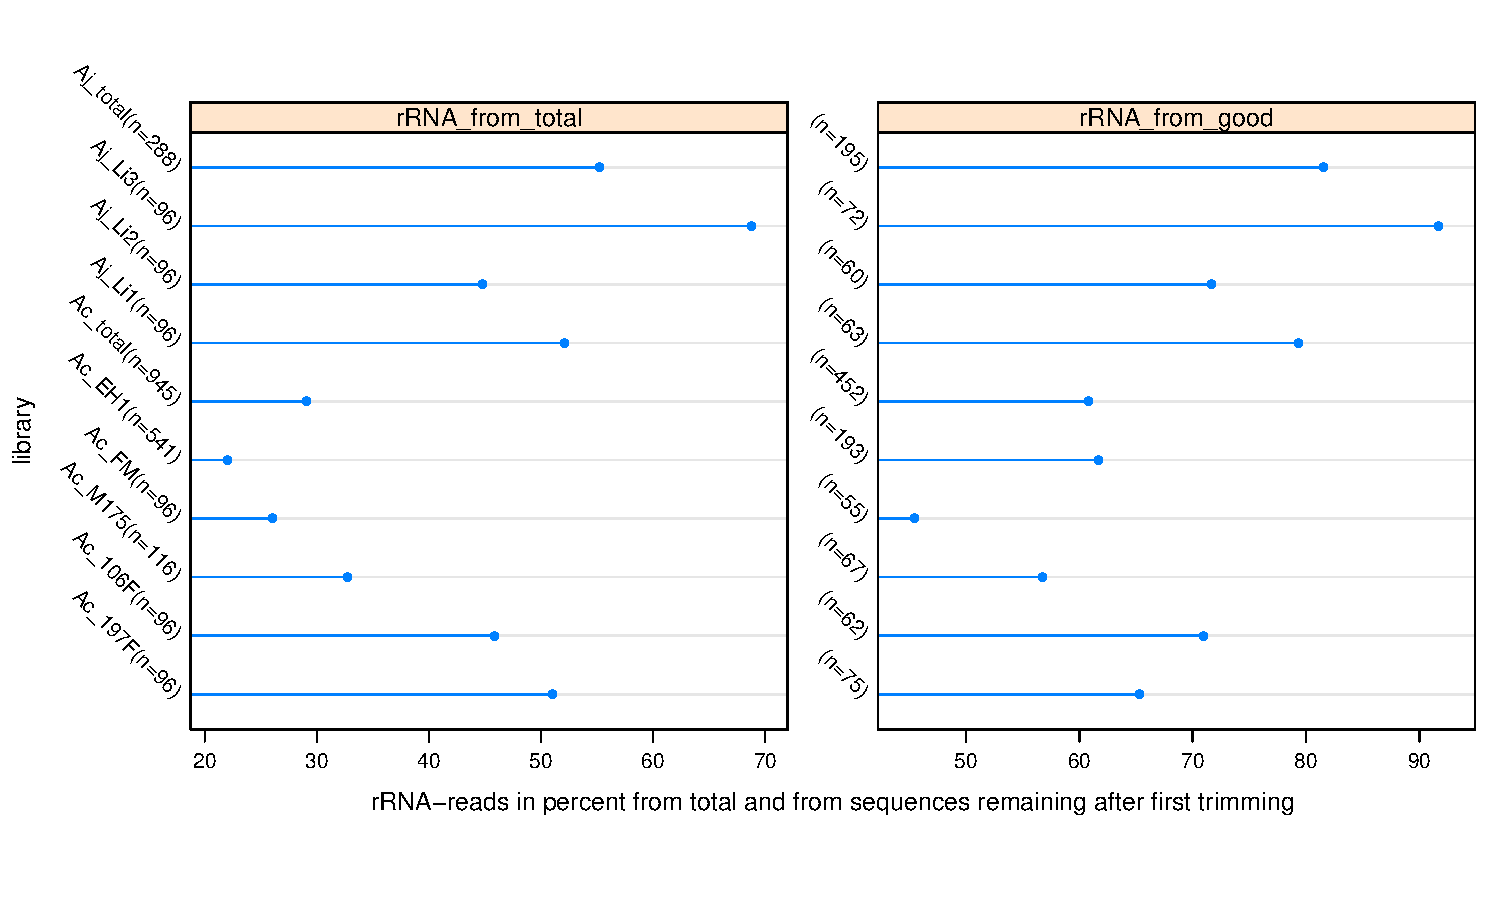
\includegraphics{pilot-006}
\caption{Proportion of rRNA contamination in different libraries for
  \textit{A. crassus}.}
\label{fig:rRNA}
\end{figure}


\subsection*{Screening for host-contamination)}

The GC-content of \textit{A. crassus} ESTs gave first pointers on
possible contamination still left in the sequences after these
steps. \textit{A. crassus} had a lower mean GC-content (p < 0.001)
NA
mean $\pm$ sd) than \textit{Anguilla japonica}
NA
mean $\pm$ sd). The probability density function of GC-contents
pointed on some unusual sequences containing as high as 65\% GC (see
fig. \ref{fig:GC}) in the \textit{A. crassus} set. Further inspection
of preliminary annotations from BLAST searches against NR, showed that
the first sequence with a annotation relating it to a nematode protein
was Ac\_FMf\_08A08 (the sequence with the 8th highest GC-content), for
which similarity to "collagen col-34" from \textit{Brugia malayi} was
inferred.

\begin{figure}[ht]
  \centering \advance\leftskip-2.275cm
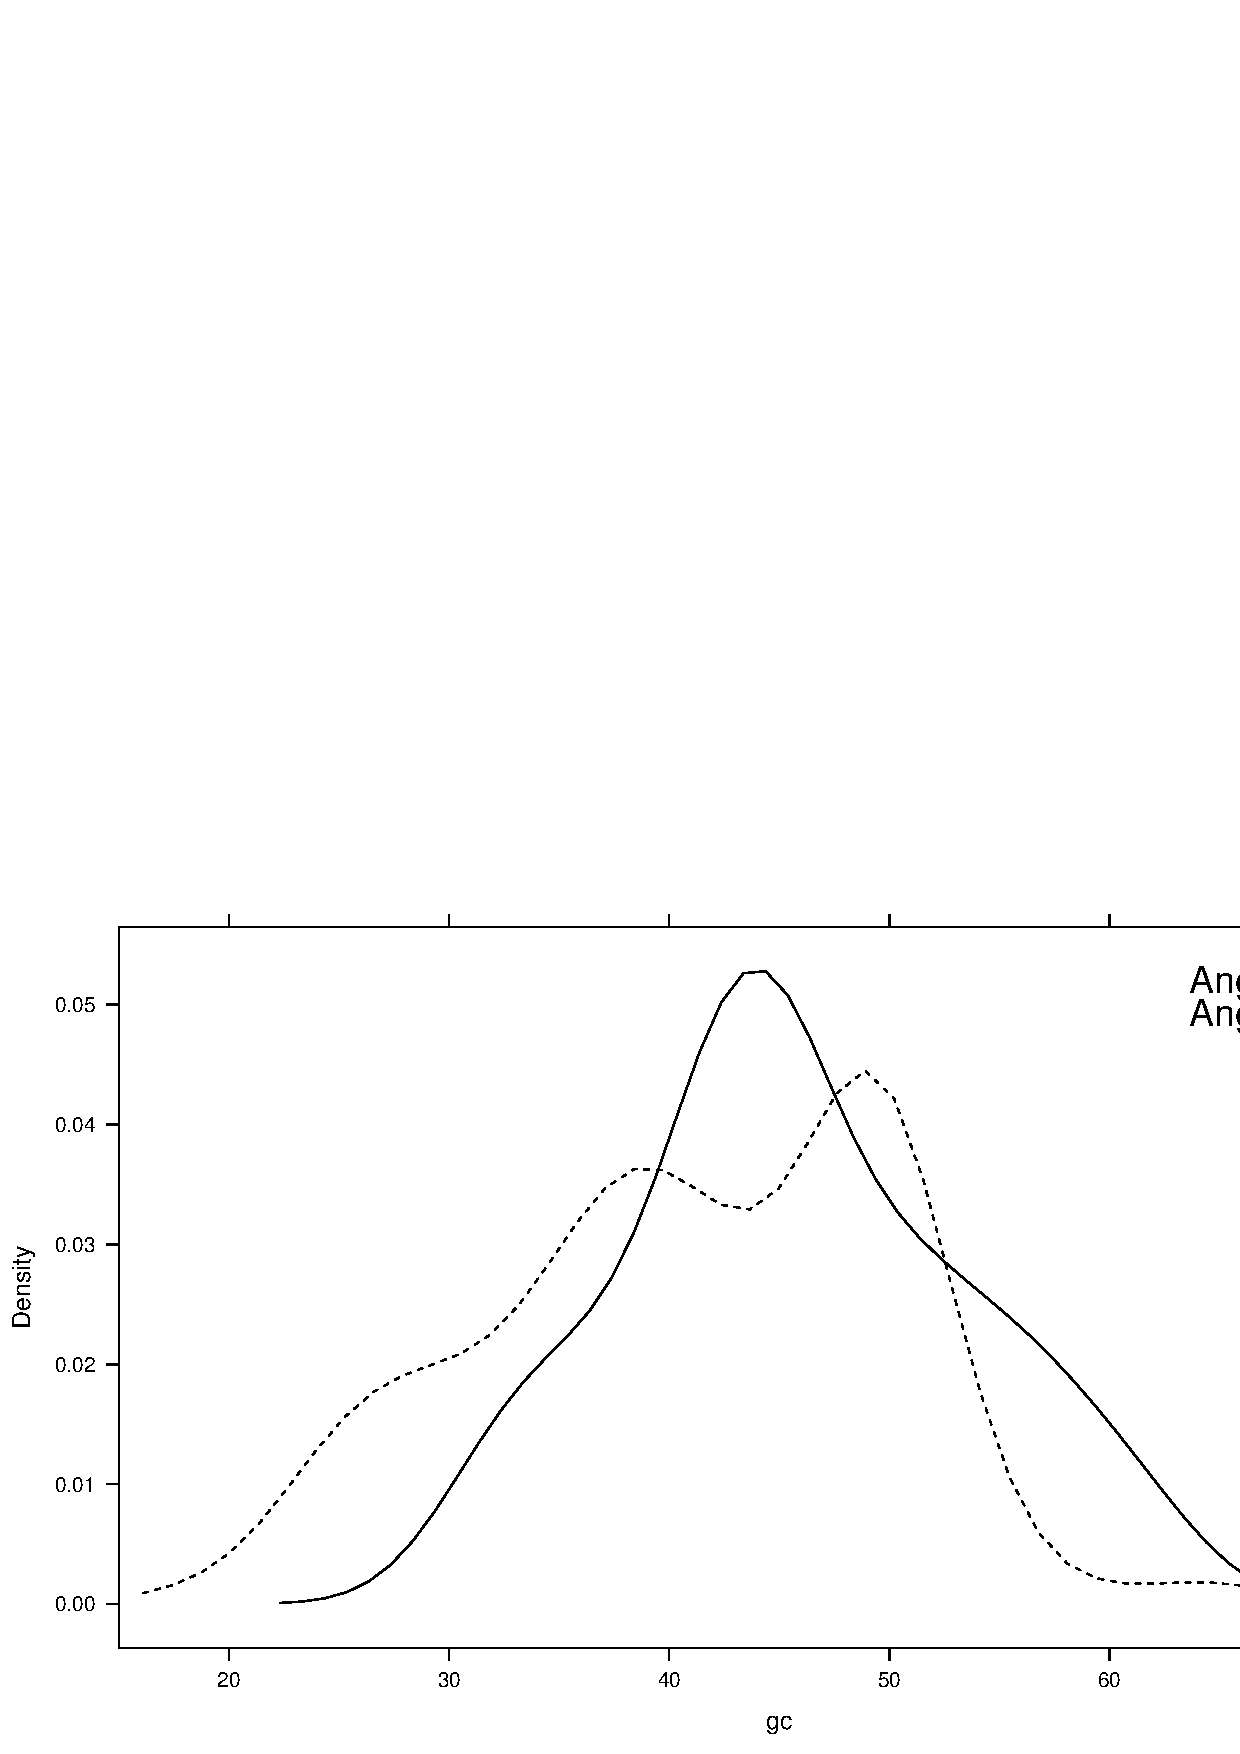
\includegraphics{pilot-008}
\caption{GC-content of sequences from \textit{Anguilla japonica} and
  \textit{A.crassus}.}
\label{fig:GC}
\end{figure}

Manual inspection of the remaining annotations made clear that another
filtering for host sequences was necessary (3 sequences had best BLAST
hits to proteins from non-teleost vertebrates, 7 from teleosts). A
comparison of BLAST results for these sequences versus nempep4 and a
fishprotein database (derived from NCBI non-redundant), showed that
they were more likly to originate from host contamination than from
\textit{A. crassus} (see table \ref{tab:hostex}). They were excluded
from the submission file, reducing the number of sequences for
submission to 113.

\begin{table}[ht]
  \centering
  \begin{tabular}{llll} 
    EST&fishpep annotation&evalue\\
    \hline
    Ac\_106F\_01A06& PREDICTED: similar to FAT tumor&1.00E-017\\
    &suppressor homolog 4 [Danio rerio]\\
    Ac\_EH1\_01C10 &Ferritin,  middle subunit       &2.00E-088  \\ 
    & [Salmo salar]                    \\ 
    Ac\_EH1\_009C03&hypothetical protein LOC567037  &7.00E-037  \\ 
    & [Danio rerio]                    \\ 
    Ac\_EH1\_01A02&muscle-specific beta 1 integrin  &2.00E-091  \\ 
    &binding protein 2 [Epinephelus      \\ 
    &coioides]                           \\ 
    Ac\_EH1\_01A07&RecName: Full = Hemoglobin anodic  &2.00E-076  \\ 
    &subunit beta; AltName:            \\ 
    &Full = Hemoglobin anodic beta chain \\ 
    Ac\_M175\_01B06&lrrc15 [Danio rerio]            &2.00E-016  \\ 
    Ac\_FM\_08F03 &PREDICTED: similar to stromal    &2.00E-057  \\ 
    &antigen 2 isoform 1 [Danio rerio] \\ 
    Ac\_M175\_01H02&Peroxiredoxin-1 [Salmo salar]   &1.00E-101  \\ 
    Ac\_EH1\_005B07&cyclin G1 [Poecilia reticulata] &9.00E-019  \\ 
    Ac\_EH1\_005B07&Cyclin G1 [Danio rerio]         &1.00E-011  \\ 
    \hline 
\end{tabular}   
\caption{Sequences excluded because of inferred "host-like" annotation}
\label{tab:hostex}
\end{table}

Sequences (forward and reverse) from Ac\_EH1\_01D10 which possibly are
derieved from bacterial contaminarion, were left in the
submission-file, because it could not be fully excluded that they
originated from symbiotic bacteria.

Anoter sequence for wich a xenobiotic origin seems pessible is
Ac\_FM\_08D01 annotated as "putative senescence-associated protein"
from the plant \textit{Pisum sativum}.

\section*{Discussion}

A total of  sequencing-reads from
\textit{A. crassus} (4 different libraries) and
 reads from liver tissue (3 libraries)
of the host species \textit{Anguilla japonica} resulted in
115 nematode- and
36 host quality ESTs submittable to NCBI
dbEST. The low proportion of high quality ESTs is mainly a result of a
high degree of rRNA contamination present in all libraries and of the
fact that 40\% of the sequencing rections for
\textit{Anguillicoloides} were prepared by unexperienced undergraduate
students in the framework of a practical.

The high proportion of rRNA in the host-ESTs clearly shows, that
shortcomings in the preparation of cDNA rather than sequence-specific
difficulties are responsible for this contamination.

A minor fraction of reads had to be excluded because of
sequencing-reactions starting at a poly-A tail producing artificial
homopolymer-runs. The basic regular expression used for this purpose
produced good results identifying only two sequences, which had a hit
to protein annotated by blast similarity within nempep4 wrongly (false
positives). Another evitable false positive had a hit to a nempep4
protein transcribed by ESTscan\cite{estscan} within PArtigene. Visual
inspection of this sequence led to the conclusion, that not the
classification as artificial inferred here is likely to be wrong, but
rather nembase4 contains an artificial low-complexity sequence leading
to a blast-hit. Nevertheless the method for filtering of these
seqences could still be improved further by designing a more
sofisticated algorithm, that e.g. assigns different penalty-scores to
homopolymer-runs of different length and excludes sequences of a
certain penalty-score per length.

After exclusion of low quality and rRNA sequences the remaining
sequences from \textit{A. crassus} had to be examined for host
contamination.The present analysis showed that examination of
GC-content is a powerful tool for this purpose in \textit{A. crassus}
transcriptome sequences.The 7 sequences with the highest GC-contents
contained six sequences that had to be removed from the submission
file because of an annotation making a host origin likely. In total 10
sequences had to be excluded.

This amount of host-contamination is rather high compared to other
nematode EST studies. Nevertheless given the large proportion of host
blood ingested by \textit{A. crassus} compared to the small nematode
itself, such a contamination is not too suprising.

%%%%%%%%%%%%%%%%%%%%%%%%%%%%%%%%%%%%%%%%%%%%%%%%%%%%%%%%%%%%%
%%                  The Bibliography                       %%
%%                                                         %%              
%%  Bmc_article.bst  will be used to                       %%
%%  create a .BBL file for submission, which includes      %%
%%  XML structured for BMC.                                %%
%%                                                         %%
%%                                                         %%
%%  Note that the displayed Bibliography will not          %% 
%%  necessarily be rendered by Latex exactly as specified  %%
%%  in the online Instructions for Authors.                %% 
%%                                                         %%
%%%%%%%%%%%%%%%%%%%%%%%%%%%%%%%%%%%%%%%%%%%%%%%%%%%%%%%%%%%%%


\bibliographystyle{/home/ele/bibtex/bmc_article.bst} % Style BST file
\newpage
\bibliography{/home/ele/bibtex/master.bib} % Bibliography file (usually '*.bib' )



%%%%##########################################################################

\end{document}

% LocalWords: transcriptome Anguillicoloides crassus ESTs
% coreresponding LocalWords: Heitlinger swimbladder japonica NCBI
% dbEST rRNA againt
